\chapter{Arhitektura i dizajn sustava}
	{Arhitektura cijelog sustava može se podijeliti na četiri ključna dijela:}
		\begin{itemize}
    		\item Web preglednik
    		\item Web aplikacija
    		\item Baza podataka
    		\item Code runner
		\end{itemize}

	{\underline{Web preglednik} omogućuje interakciju između korisnika i aplikacije. Svaki se korisnikov zahtjev
	 događa na web pregledniku i prosljeđuje aplikaciji na obradu. Osim slanja zahtjeva, korisniku se omogućuje
	  bolji pregled aplikacije pomoću apstraktnog koda kojeg web preglednik pretvara u lako shvatljive strukture.}\\

	{\underline{Aplikacija} se sastoji od tri  servisa, frontenda, API servisa i evaluatora. Tehnologije koje se koriste na backendu
	 uključuju programski jezik \textbf{Python} i \textbf{FastApi} web framework koji omogućuje stvaranje aplikacije temeljene na \textbf{REST}
	 arhitekturi i rutera na kojem su definirane rute za slanje zahtjeva i komunikaciju korisnika i aplikacije.
	 Frontend aplikacije izrađen je korištenjem libraryja \textbf{React}, a kod je pisan u \textbf{TypeScriptu}. On omogućuje korisniku jednostavan pregled
	 aplikacije i jednostavno korištenje aplikacije, odnosno slanje zahtjeva.}\\

	{\underline{Kontejneri} se koriste unutar aplikacije kako bi poboljšali korisničko iskustvo, optimizirali performanse sustava
	te osigurali skalabilnost za povećani broj korisnika. Glavni se dio aplikacije s ruterima i logikom za komunikaciju s 
	bazom nalazi u vlastitom kontejneru kao i glavna baza, evaluator i blob storage.}\\

	{Za primarnu \underline{bazu podataka} koristi se \textbf{PostgreSQL}. Primarna baza se nalazi u vlastitom kontejneru kojemu backend
	aplikacije pristupa kako bi spremio informacije u nju. Na backendu se koristi \textbf{psycopg} PostgreSQL adapter koji omogućuje
	komunikaciju između baze i backenda.}\\
	
	{\underline{Evaluator} komunicira s vanjskim \underline{Code runnerom} za kompajliranje kodova koje korisnik šalje
	na backend. Ovaj ključni dio sustava odgovoran je za izvršavanje kôda unutar sigurnog okruženja, čime se osigurava
	izolacija korisničkih skripti od ostatka aplikacije. Kroz ovu komunikaciju, Evaluator prima kôd od korisnika,
	proslijeđuje ga Code runneru na izvršavanje te zatim interpretira rezultate kako bi ih pravilno integrirao
	natrag u aplikaciju.}

	{Dodatno, evaluator koristi \textbf{blob storage} (Azure blob storage) pomoću kojeg dohvaća podatke koji su mu potrebni za
	evaluaciju određenog zadatka. Evaluator ima pristup informacijama poput ulaznih podataka za testiranje,
	očekivanih rezultata te drugih specifičnih parametara vezanih uz pojedini zadatak.}
	
	\newpage
	
		

		

				
		\section{Baza podataka}
		
		Za implementaciju našeg sustava koristit ćemo PostgreSQL, relacijsku bazu podataka. Ovaj tip baze podataka posebno je pogodan za modeliranje kompleksnih struktura koje odražavaju realni svijet, zahvaljujući svojoj sposobnosti da efikasno upravlja relacijama, odnosno tablicama. Svaka tablica u bazi unikatno je definirana svojim nazivom i skupom atributa, čime se omogućava precizno strukturiranje podataka. Jedna od ključnih prednosti PostgreSQL baze je njena brzina i efikasnost u obradi podataka, uključujući pohranu, ažuriranje i dohvaćanje informacija. Naša baza podataka obuhvatit će niz entiteta koji su specifično prilagođeni zahtjevima naše aplikacije.
		
		\textit{Popis entiteta: users, competitions, problems, competition\_participations, problems\_on\_competitions, 
			problem\_results, trophies i verification\_tokens.}
		
		
		\eject
		\subsection{Opis tablica}
		
		
		\subsubsection*{Users}
		
		Entitet \textbf{users} sadržava sve važne informacije o korisniku aplikacije. Sadrži atribute: \textit{id, role, username, image\_url, password\_hash, email, name, surname, is\_verified, created\_on}. 
		Ovaj entitet je u \textit{many-to-many} vezi s entitetom \textit{competitions} preko tablice \textit{competition\_participations}. Ovaj entitet je u \textit{one-to-many} vezi s entitetom \textit{verification\_tokens} preko atributa \textit{email}. 
		
		\begin{figure}[htbp]
			\centering
			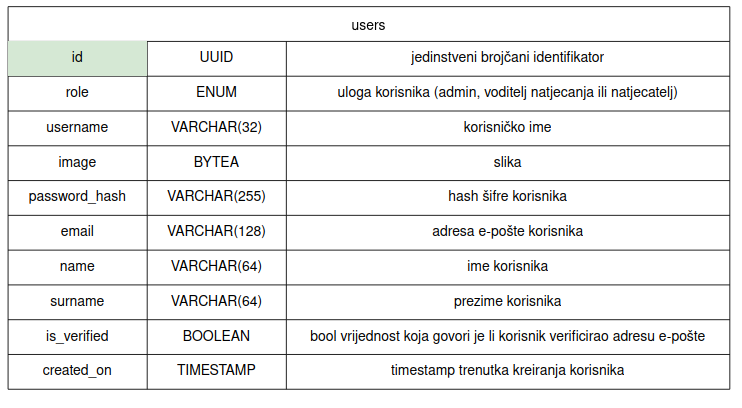
\includegraphics[width=\linewidth]{slike/users_tablica.png}
			\caption{Entitet \textbf{users}}
		\end{figure}
		\eject
		
		\subsubsection*{Problems}
		
		Entitet \textbf{problems} sadržava sve važne informacije o zadacima. Sadržava atribute: \textit{id, name, description, example\_input, example\_output, is\_hidden, num\_of\_points, runtime\_limit, tests\_dir, is\_private, created\_on}. Ovaj entitet je u \textit{many-to-many} vezi s entitetom \textit{competitions} preko tablice \textit{problems\_on\_competitions}. Ovaj entitet je u \textit{one-to-many} vezi s entitetom \textit{problem\_results} preko atributa \textit{id}.
		
		\begin{figure}[htbp]
			\centering
			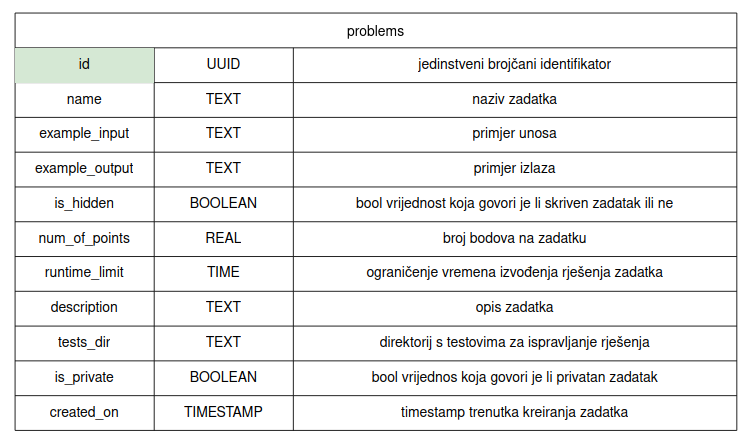
\includegraphics[width=\linewidth]{slike/problems_tablica.png}
			\caption{Entitet \textbf{problems}}
		\end{figure}
		\eject
		
		\subsubsection*{Competitions}
		
		Entitet \textbf{competitions} sadržava sve važne informacije o natjecanjima. Sadržava atribute: \textit{id, name, description, start\_time, end\_time, parent\_id, problems}. Natjecanja mogu imati svoja nadređena natjecanja. Ovaj entitet je u \textit{many-to-many} vezi s entitetom \textit{users} preko \textit{competition\_participations} tablice. Ovaj entitet je u \textit{many-to-many} vezi s entitetom \textit{problems} preko \textit{problems\_on\_competitions} tablice.
		
		\begin{figure}[htbp]
			\centering
			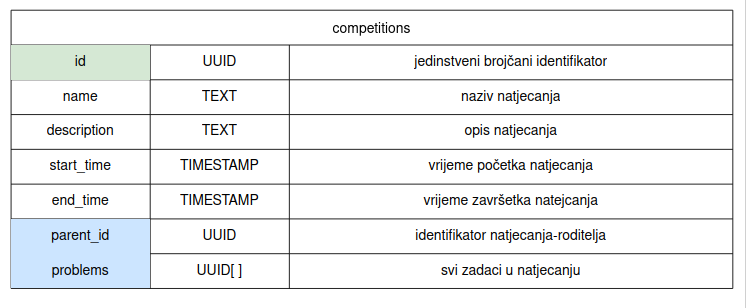
\includegraphics[width=\linewidth]{slike/competitions_tablica.png}
			\caption{Entitet \textbf{competitions}}
		\end{figure}
		
		\subsubsection*{Competition\_participations}
		
		Entitet \textbf{competition\_participations} sadržava sve važne informacije o sudjelovanju korisnika na natjecanjima. Sadržava atribute: \textit{id, user\_id, competition\_id, num\_of\_points}. Ovaj entitet je u \textit{many-to-many} vezi s entitetom \textit{users}. Ovaj entitet je u \textit{many-to-many} vezi s entitetom \textit{competitions} preko atributa \textit{competition\_id}.
		
		\begin{figure}[htbp]
			\centering
			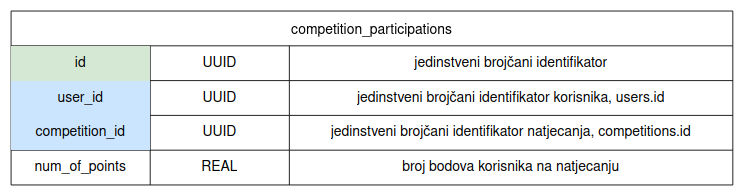
\includegraphics[width=\linewidth]{slike/competition_participations_tablica.png}
			\caption{Entitet \textbf{competition\_participations}}
		\end{figure}
		
		\subsubsection*{Problems\_on\_competitions}
		
		Entitet \textbf{problems\_on\_competitions} sadržava informacije o zadacima koji pripadaju pojedinim natjecanjima. Sadržava atribute: \textit{id, problem\_id, competition\_id, num\_of\_points}.
		
		\begin{figure}[htbp]
			\centering
			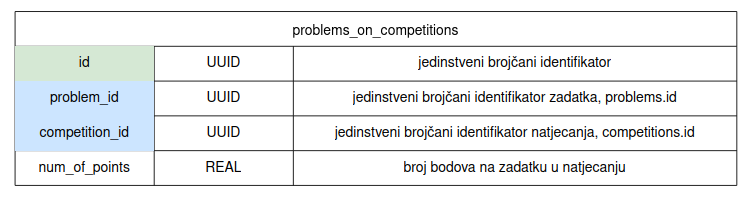
\includegraphics[width=\linewidth]{slike/problems_on_competitions_tablica.png}
			\caption{Entitet \textbf{problems\_on\_competitions}}
		\end{figure}
		
		\eject
		
		\subsubsection*{Problem\_results}
		
		Entitet \textbf{problem\_results} sadrži rezultate pojedinih korisnika na pojedinim zadacima. Sadržava atribute: \textit{id, user\_id, problem\_id, competition\_id, num\_of\_points, average\_runtime, is\_correct, source\_code}. Ovaj entitet je u \textit{one-to-many} vezi s entitetom \textit{users} preko \textit{user\_id} te \textit{one-to-many} vezi s entitetom \textit{problems} preko atributa \textit{problem\_id}. Ovaj entitet je u \textit{one-to-many} vezi s entitetom \textit{competitions} preko atributa \textit{competition\_id}.
		
		\begin{figure}[htbp]
			\centering
			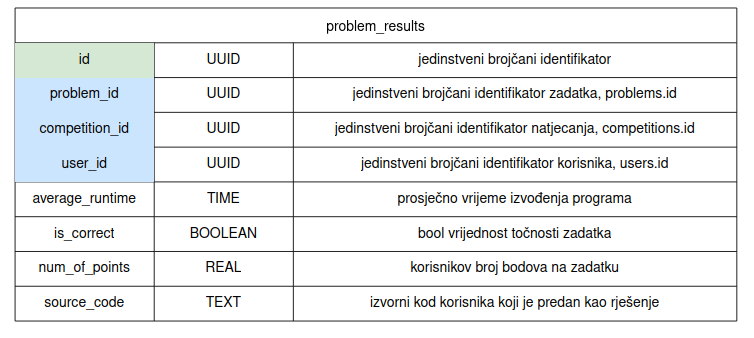
\includegraphics[width=\linewidth]{slike/problem_results_tablica.png}
			\caption{Entitet \textbf{problem\_results}}
		\end{figure}
		
		\eject
		
		\subsubsection*{Trophies}
		
		Entitet \textbf{trophies} sadržava informacije o trofejima koje korisnici mogu osvojiti. Sadržava atribute: \textit{id, competition\_id, user\_id, position, icon}. Ovaj entitet je u \textit{one-to-many} vezi s entitetom \textit{users} preko atributa \textit{user\_id} te \textit{one-to-many} vezi s entitetom \textit{competitions} preko atributa \textit{competition\_id}.
		
		\begin{figure}[htbp]
			\centering
			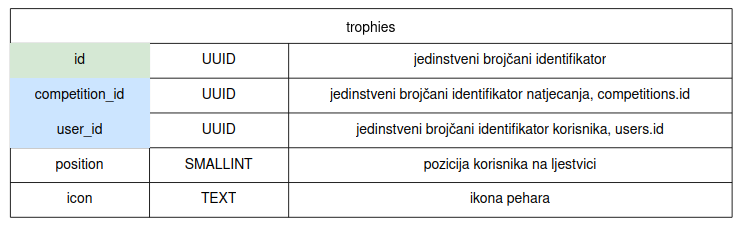
\includegraphics[width=\linewidth]{slike/trophies_tablica.png}
			\caption{Entitet \textbf{trophies}}
		\end{figure}
		
		\subsubsection*{Verification\_tokens}
		
		Entitet \textbf{verification\_tokens} sadržava informacije o tokenima za verifikaciju korisnika. Sadržava atribute: \textit{token, email, expiry\_date}. Ovaj entitet je u \textit{one-to-many} vezi s entitetom \textit{users} preko atributa \textit{email}.
		
		\begin{figure}[htbp]
			\centering
			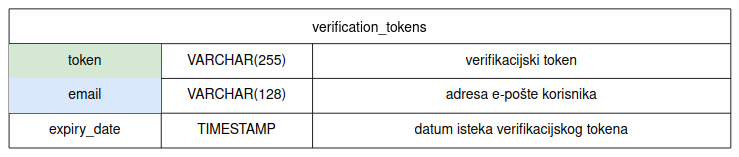
\includegraphics[width=\linewidth]{slike/verification_tokens_tablica.png}
			\caption{Entitet \textbf{verification\_tokens}}
		\end{figure}
		
		\eject
		
		\subsection{Dijagram baze podataka}
		
		
		\begin{figure}[htbp]
			\centering
			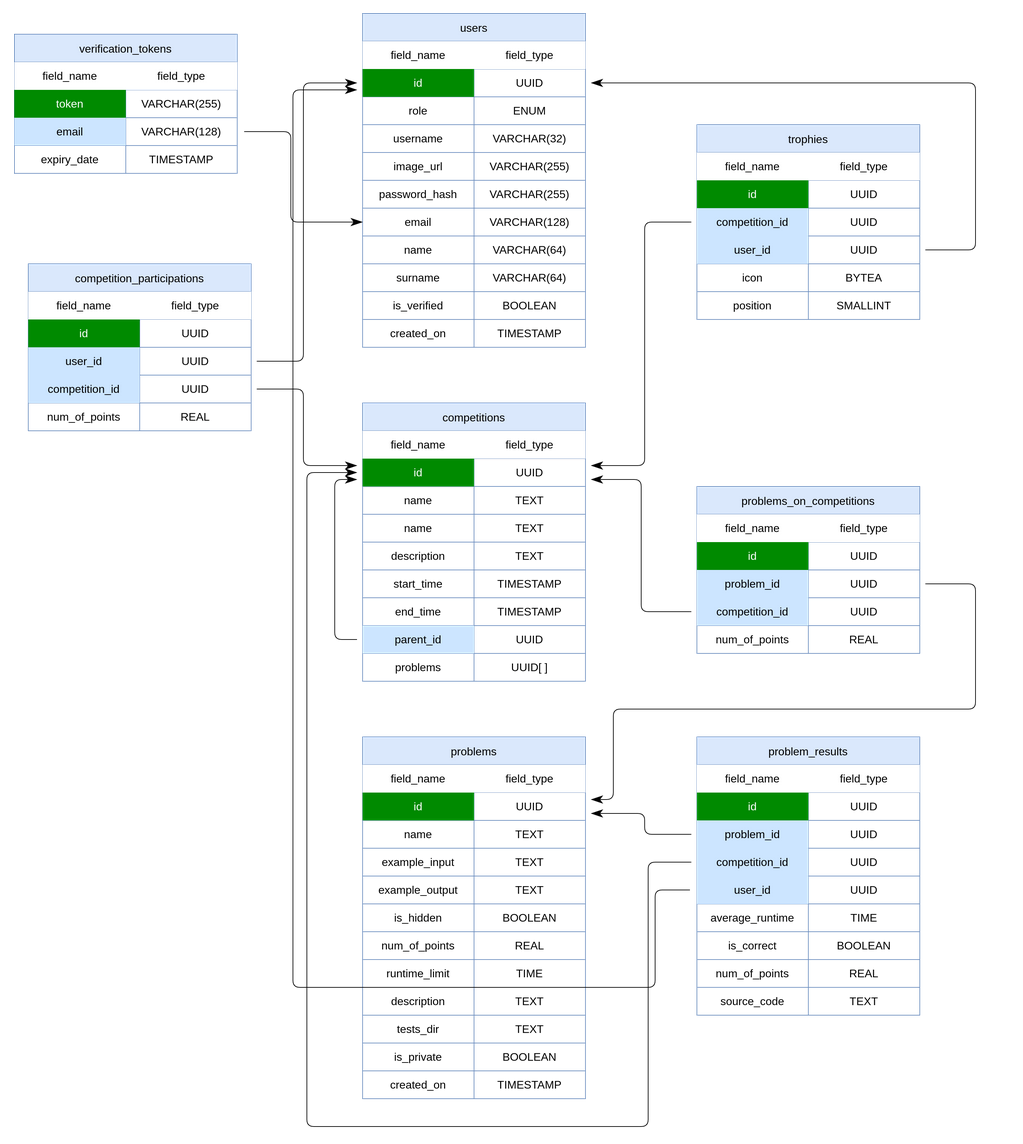
\includegraphics[scale=0.4]{slike/db_dijagram.png}
			\caption{Dijagram baze podataka}
		\end{figure}
		\eject
		
			
		\section{Dijagram razreda}
		
			
			
			Na sljedećim slikama prikazani su dijagrami razreda koji pripadaju backend dijelu aplikacije.
			
			\begin{figure}[htbp]
				\centering
				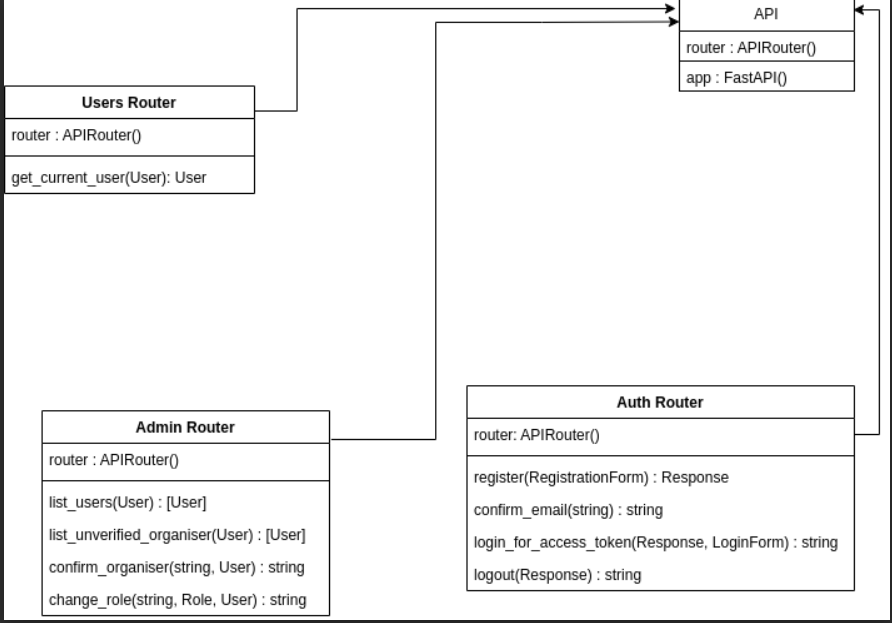
\includegraphics[width=\linewidth]{slike/dijagram_razreda.png}
			\end{figure}
			
			

			\begin{figure}[htbp]
				\centering
				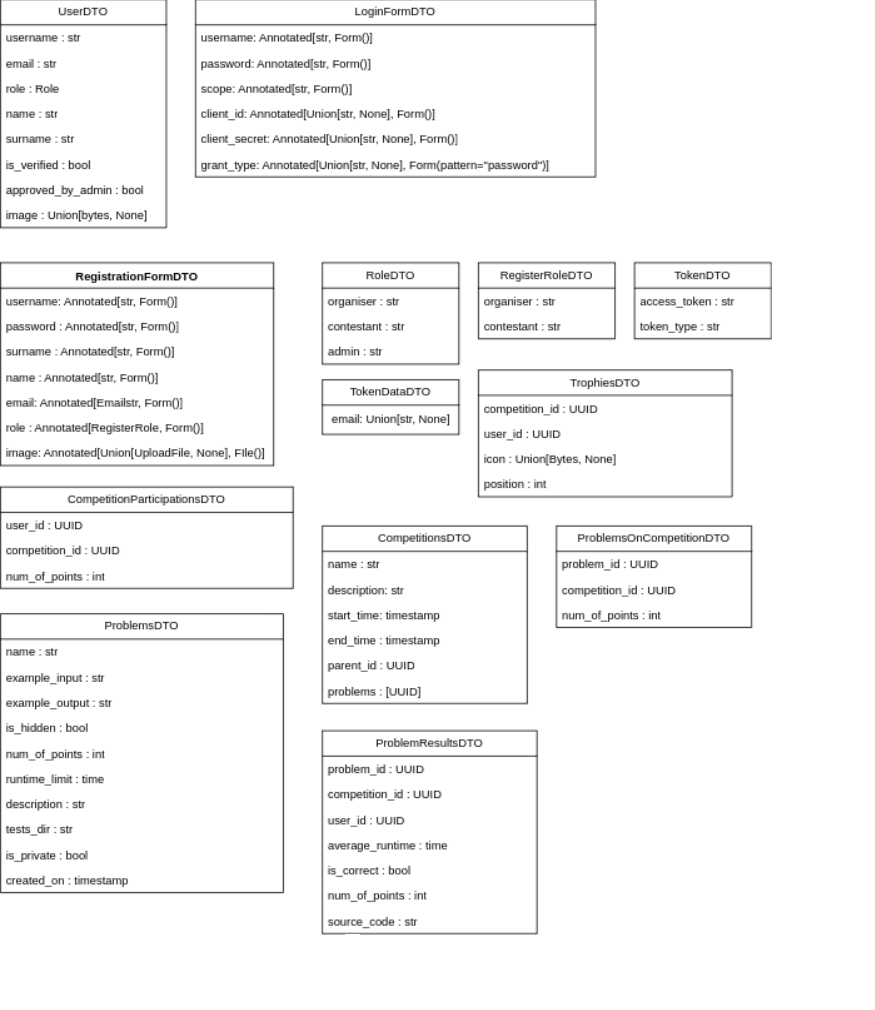
\includegraphics[width=\linewidth]{slike/dto.png}
			\end{figure}
			\eject
			
			\textbf{\textit{dio 2. revizije}}\\			
			
			\textit{Prilikom druge predaje projekta dijagram razreda i opisi moraju odgovarati stvarnom stanju implementacije}
			
			
			
			\eject
		
		\section{Dijagram stanja}

			Dijagram stanja prikazuje stanja objekta te prijelaze iz jednog stanja u drugo temeljene na događajima.
			Na slici je prikazan dijagram stanja registriranog korisnika.
			Nakon prijave, klijentu se prikazuje početna stranica na kojoj ima opciju pregleda profila natjecatelja i voditelja te opciju pregleda kalendara s natjecanjima. Nakon klika na profile natjecatelja, korisnik može pregledat njihovu statistiku sa svih natjecanja. 
			Natjecatelj može sudjelovati u natjecanju i rješavati zadatke te predati rješenje zadatka. Nakon predaje svog rješenja zadataka, ima opciju pregleda popisa svih učitanih rješenja za pojedine zadatke.
			Voditelji imaju opciju upravljanja natjecanja u kojemu mogu stvarati nova natjecanja ili kreirati nove zadatke.
			\eject
				
			\begin{figure}[H]
				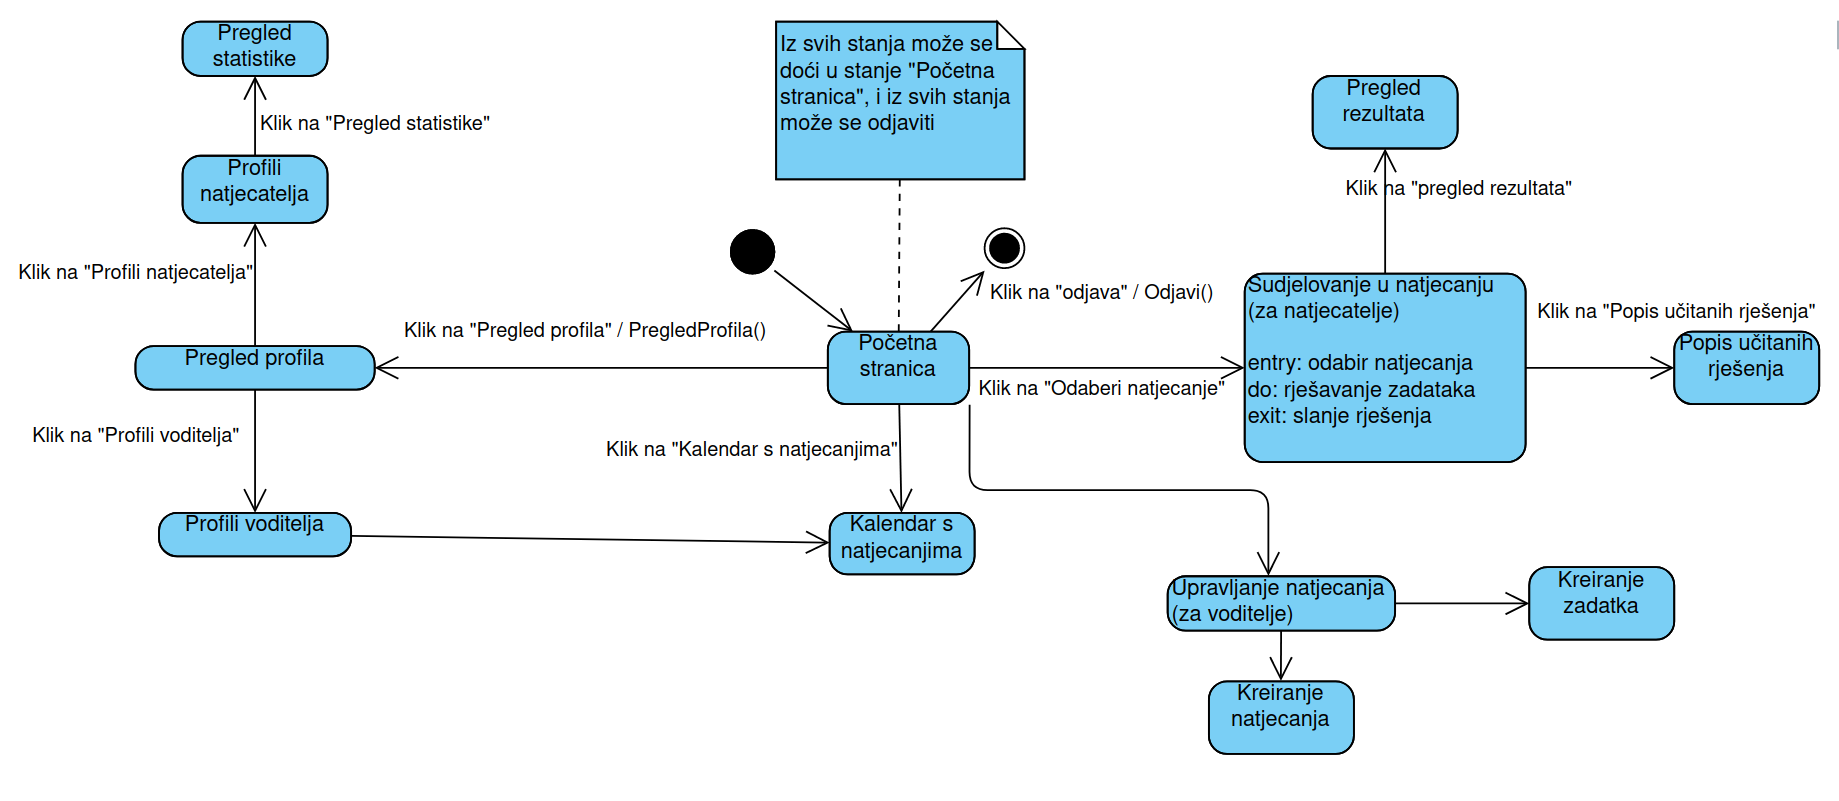
\includegraphics[width=\linewidth]{slike/dijagram_stanja.png} 
				\centering
				\caption{Dijagram stanja}
				\label{fig:stanja}
			\end{figure}
			
			\eject 
		
		\section{Dijagram aktivnosti}
			
			\textbf{\textit{dio 2. revizije}}\\
			
			 \textit{Potrebno je priložiti dijagram aktivnosti s pripadajućim opisom. Dijagram aktivnosti treba prikazivati značajan dio sustava.}
			
			\eject
		\section{Dijagram komponenti}
		
		
			Slika 4.10 prikazuje dijagram komponenti koji ilustrira kako su komponente organizirane međusobno, unutar sustava te kako su povezane s okolinom. Sustavu se pristupa kroz dva sučelja. 
			
			Prvo sučelje ima funkciju prikupljanja Typescript datoteka koje pripadaju frontend dijelu aplikacije. Ključnu ulogu ima Router, određujući koje će datoteke biti poslužene na sučelju. Frontend se sastoji od niza cjelina organiziranih prema tipovima korisnika, a Typescript datoteke koriste React, Tailwind i Primereact biblioteke za integraciju već pripremljenih komponenata.
			
			Drugo sučelje ima ulogu u preuzimanju JSON podataka i pristupanju REST API komponentama koje poslužuju podatke iz backend dijela aplikacije. DatabaseFileRetrieval zadatak ima dohvaćanje datoteka iz baze podataka korištenjem SQL upita, a zatim ti podaci putuju prema DTO-u. Reactview komponenta komunicira s ostatkom aplikacije putem dostupnih sučelja. Sustav uključuje Evaluator komponentu koja komunicira s BLOB storage-om i odgovorna je za evaluaciju rješenja zadataka. Evaulator koristi Compiler kako bi doznao ispis korisnikova koda, te ga uspoređuje sa ispravnim koji je na BLOB storage-u. Ovaj dio sustava doprinosi skalabilnosti, efikasnosti i fleksibilnosti u upravljanju podacima.
			 
			 \eject
			 
			 \begin{figure}[H]
			 	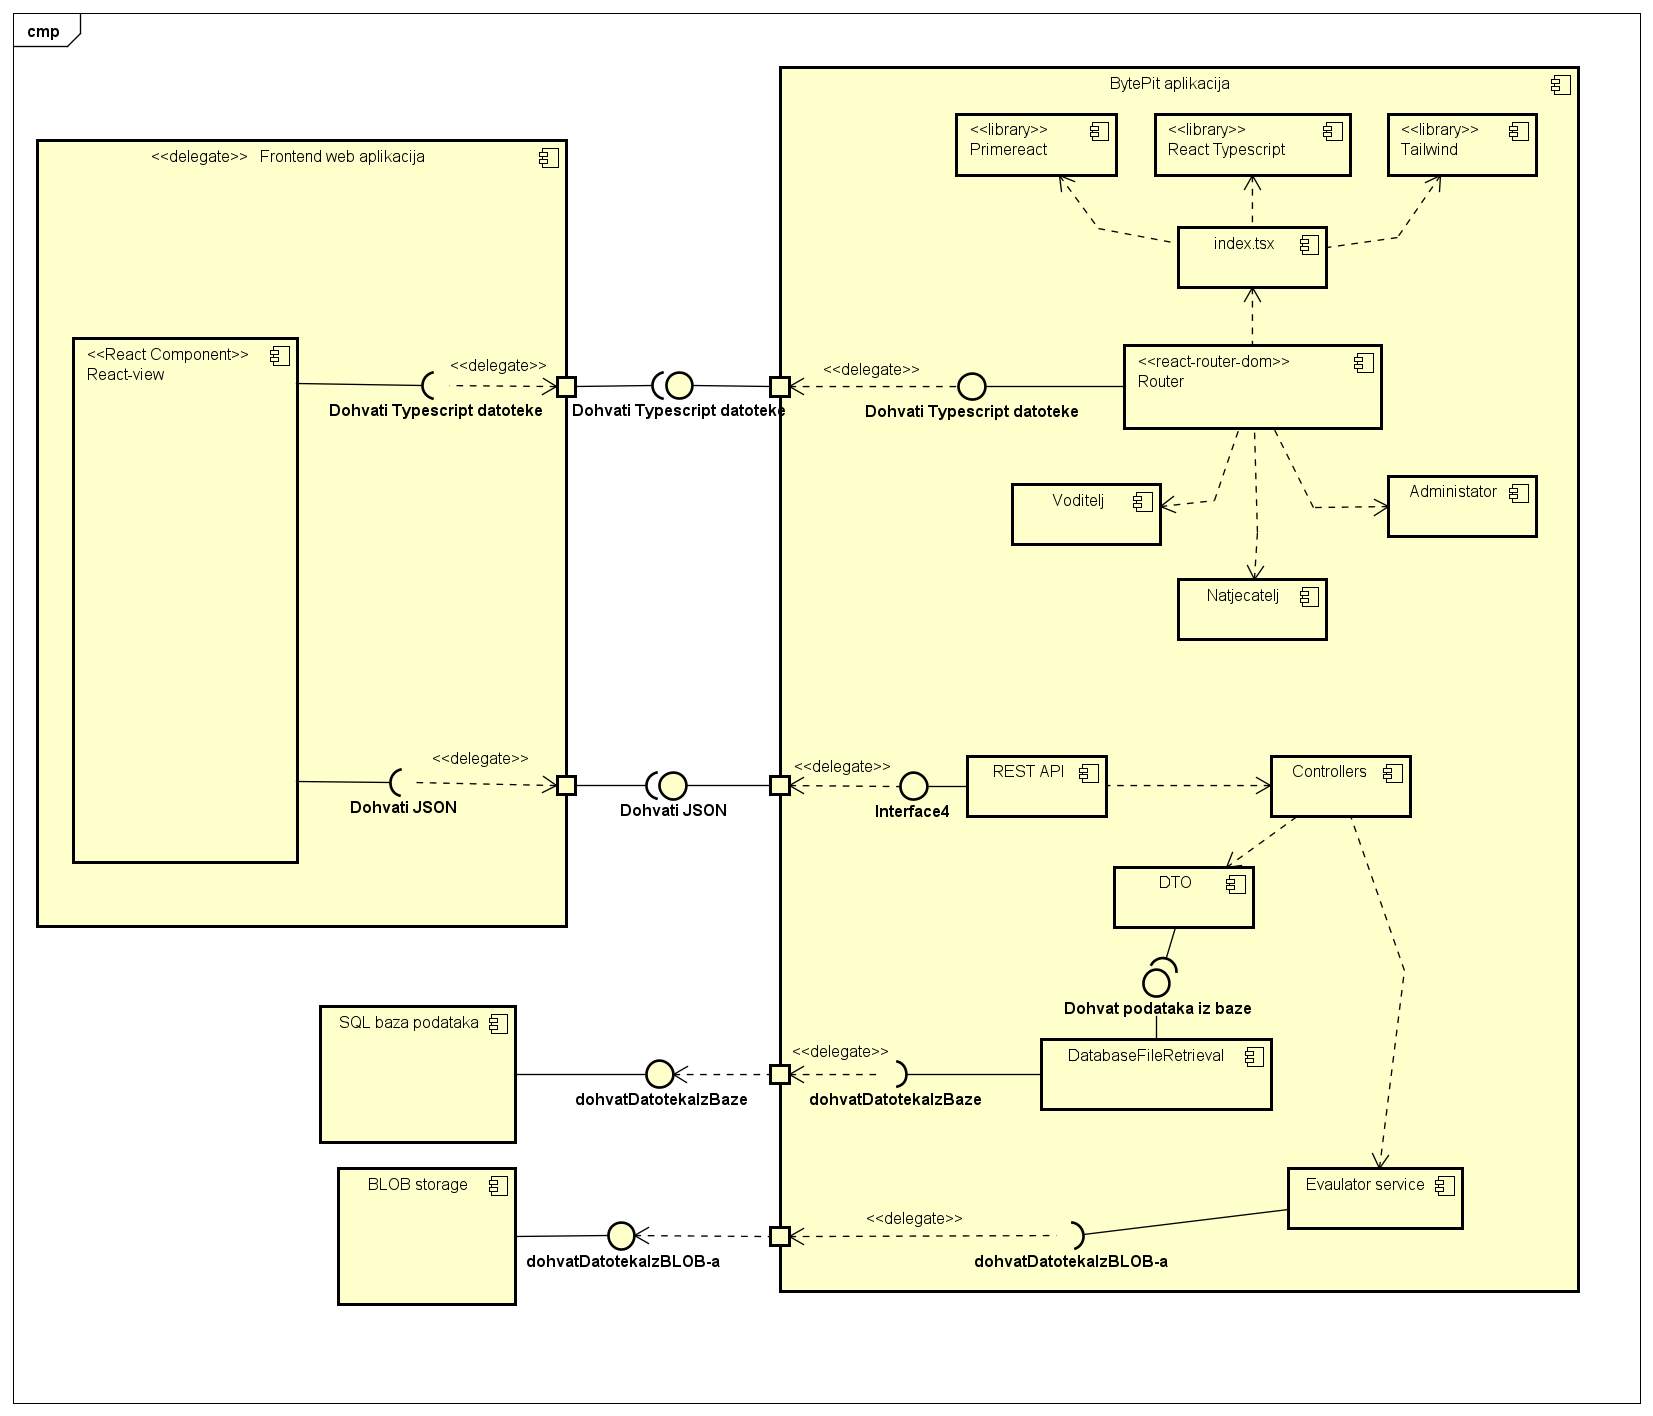
\includegraphics[scale=0.38]{slike/Dijagram_komp.PNG} %veličina slike u odnosu na originalnu datoteku i pozicija slike
			 	\centering
			 	\caption{Dijagram komponenti}
			 	\label{fig:komponente}
			 \end{figure}
			 
			 \eject